\section{Variations to the Relational Schema}
%\textcolor{red}{[Describe here variations and/or corrections to the relational schema of the previous homework, if present. Otherwise, report only the relational schema.]}

\begin{figure}[htp!]
\centering
\begin{minipage}{.5\textwidth}
  \centering
  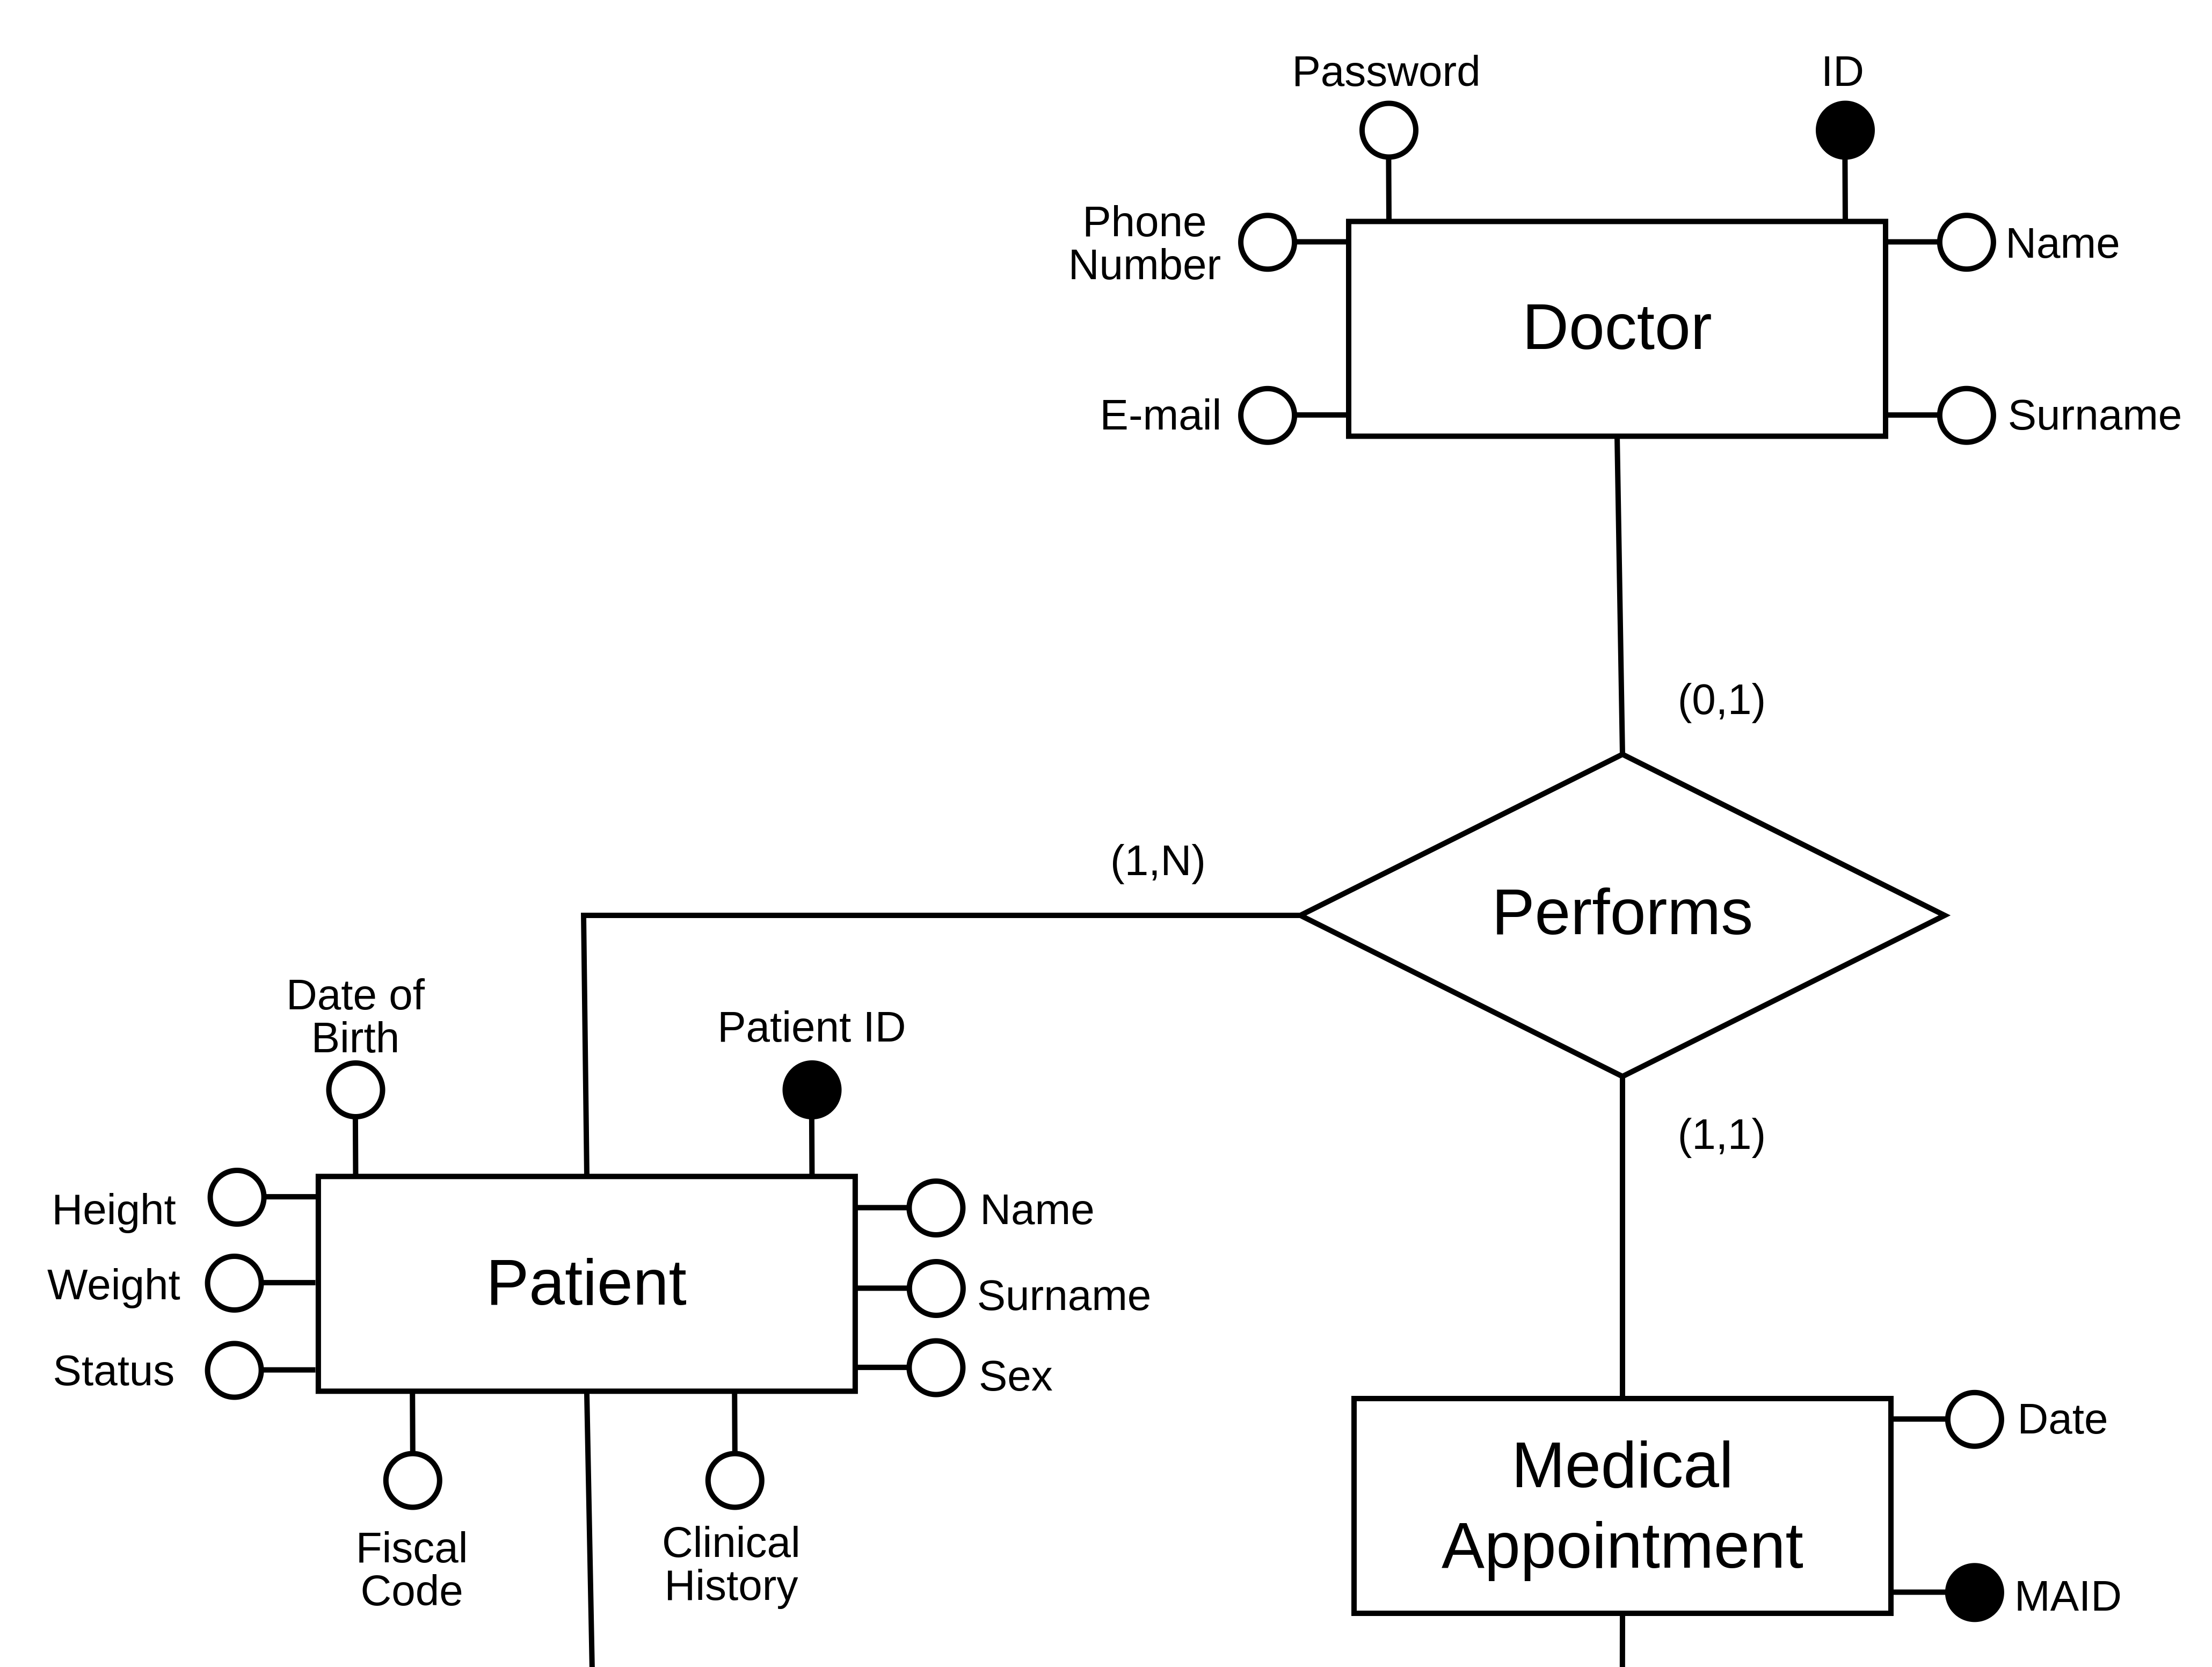
\includegraphics[width=0.725\linewidth]{schemas/er_schema_performs.png}
  \caption{Modifications of the Performs relationship}
  \label{fig:test1}
\end{minipage}%
\begin{minipage}{.5\textwidth}
  \centering
  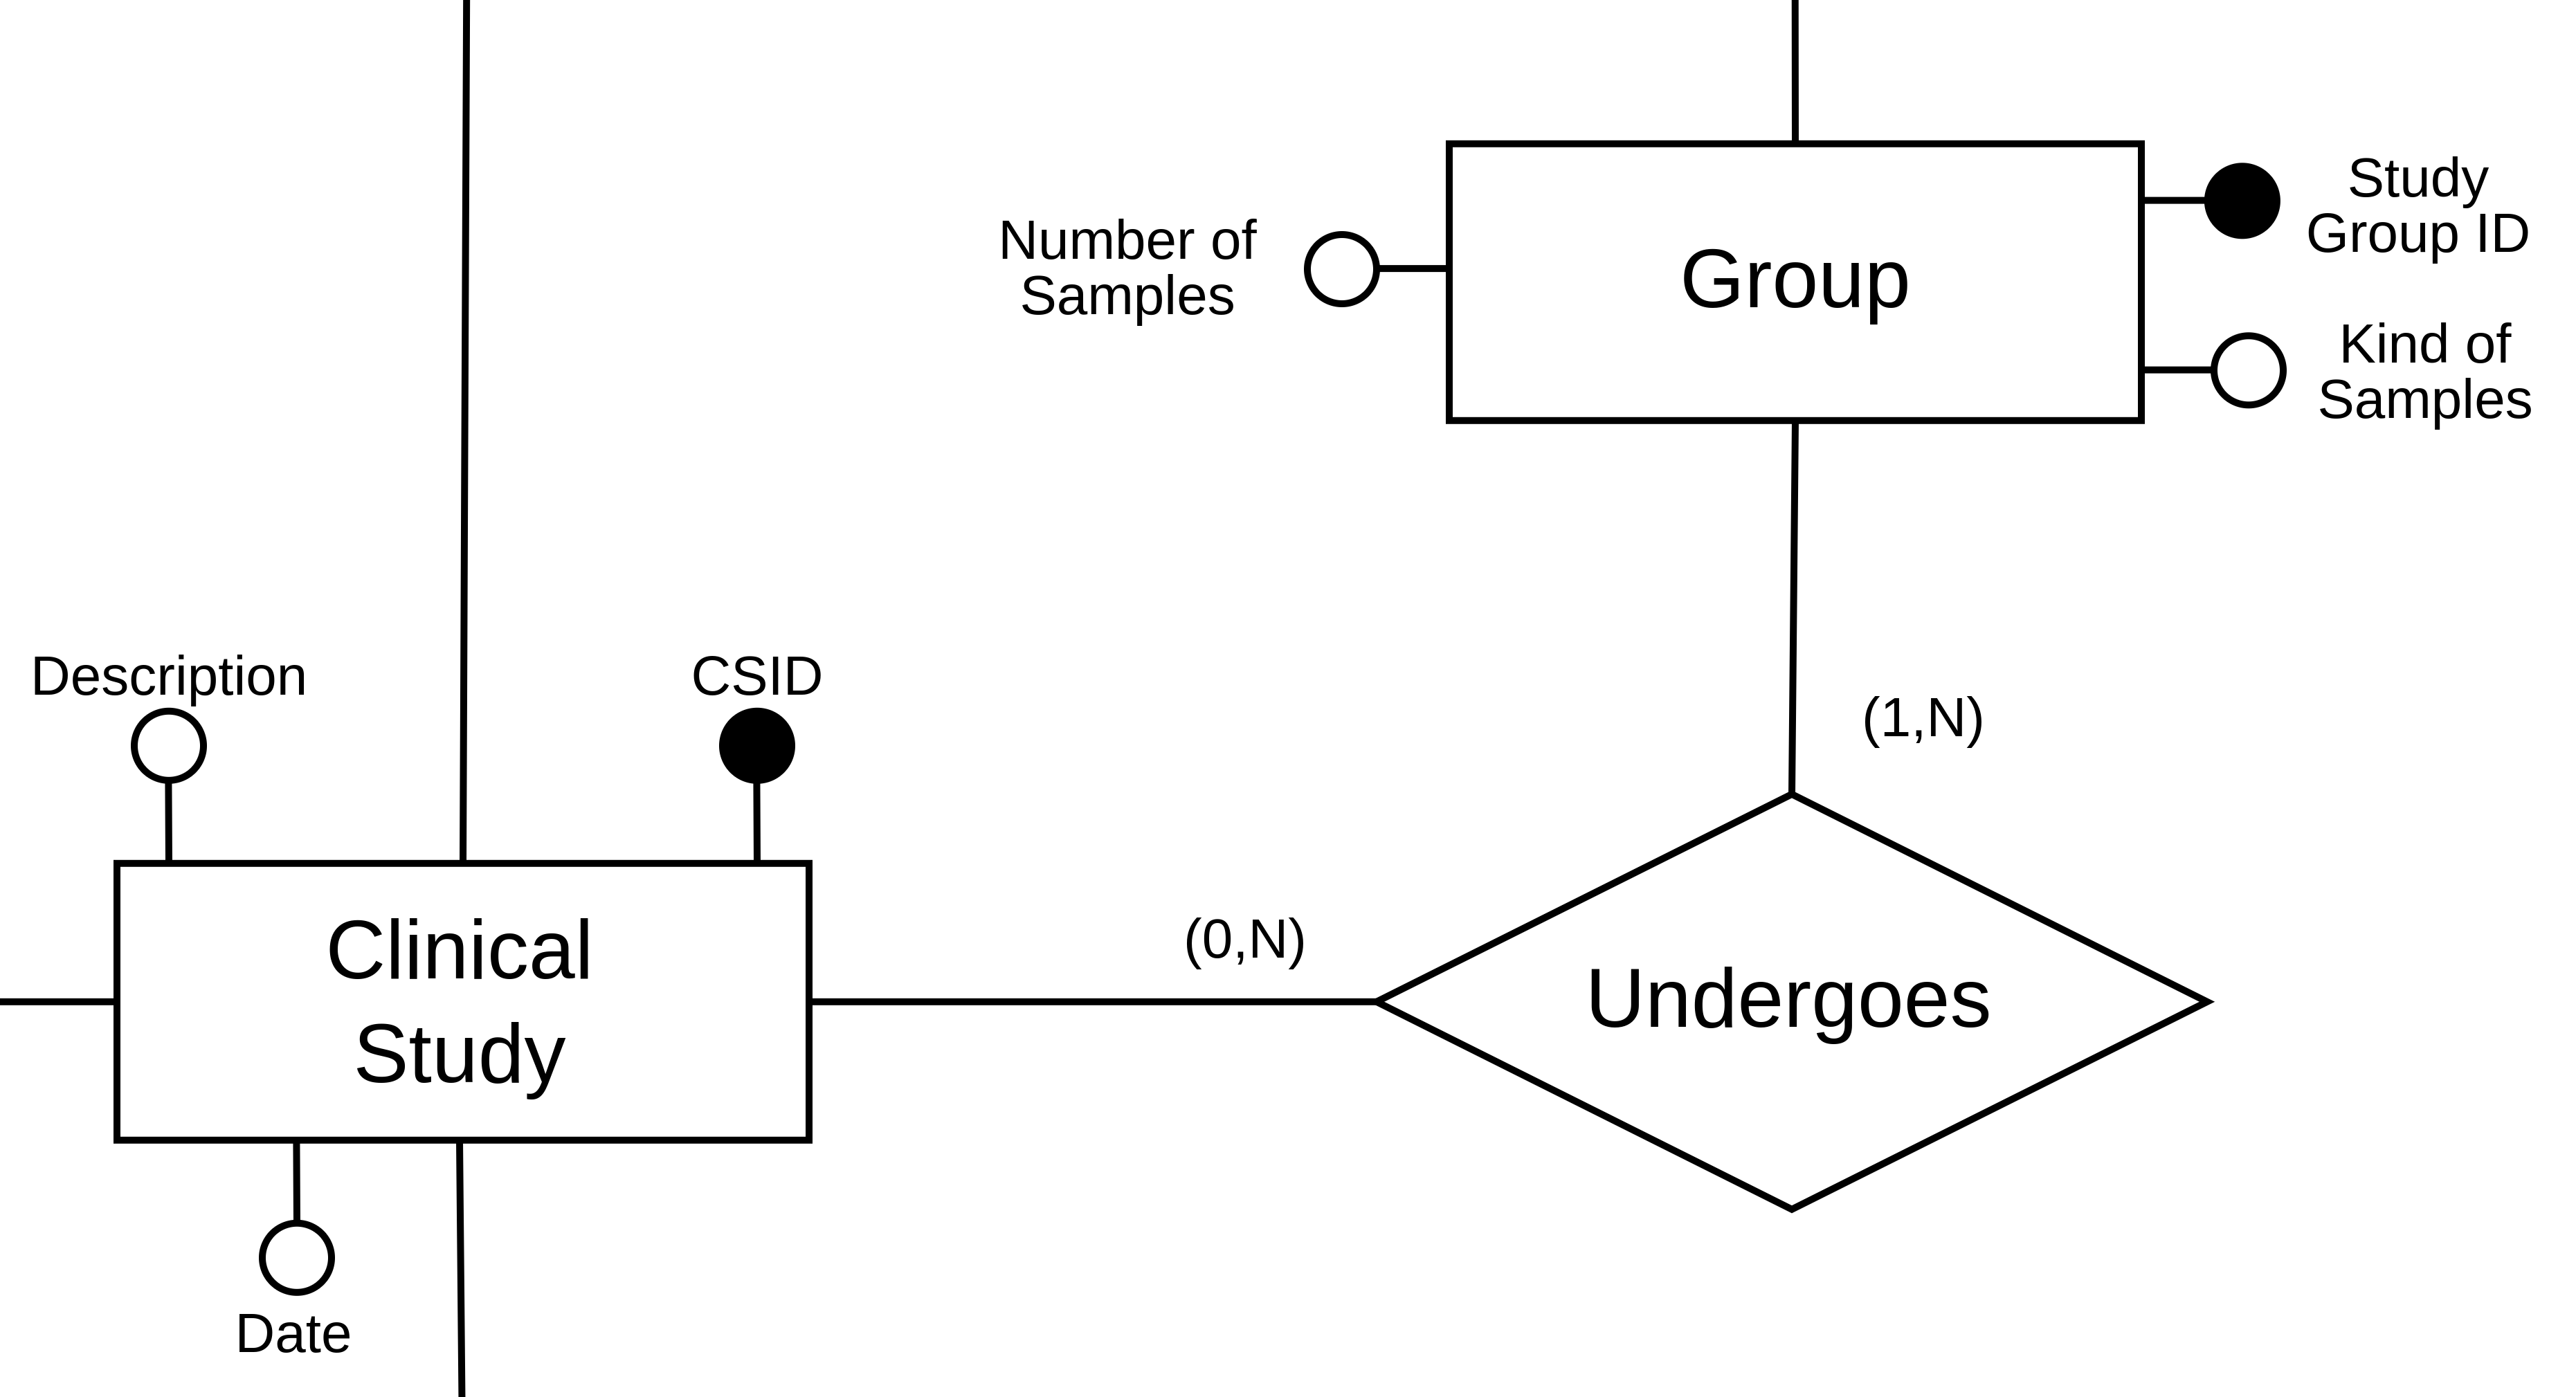
\includegraphics[width=1\linewidth]{schemas/er_schema_undergoes.png}
  \caption{Modifications of the Undergoes relationship}
  \label{fig:test2}
\end{minipage}
\end{figure}


Figure 1 and Figure 2 show the adjustments made to the entity-relationship schema, which consist in:
 \begin{itemize}
     \item Modification of the cardinality constraint involving the "Performs" relationship and the "Medical Appointment" entity from (0, N) to (1, 1), to better match the description provided in the entity table.
     \item Modification of the cardinality constraint involving the "Performs" relationship and the "Doctor" entity from (0, N) to (0, 1), thus allowing to link who was the doctor responsible for collecting the sample for the given patient.
     \item Modification of the cardinality constraint involving the "Undergoes" relationship and the "Group" entity from (0, N) to (1, N), as a group is always associated with a clinical study.
     \item Modification of the cardinality constraint involving the "Undergoes" relationship and the "Clinical Study" entity from (1, N) to (0, N), as a clinical study can be defined before having associated a group.
 \end{itemize}

 These modifications did not apport any changes to the relational schema which is depicted in Figure 3.
 \begin{center}
\begin{figure}[htp!]
    \centering
    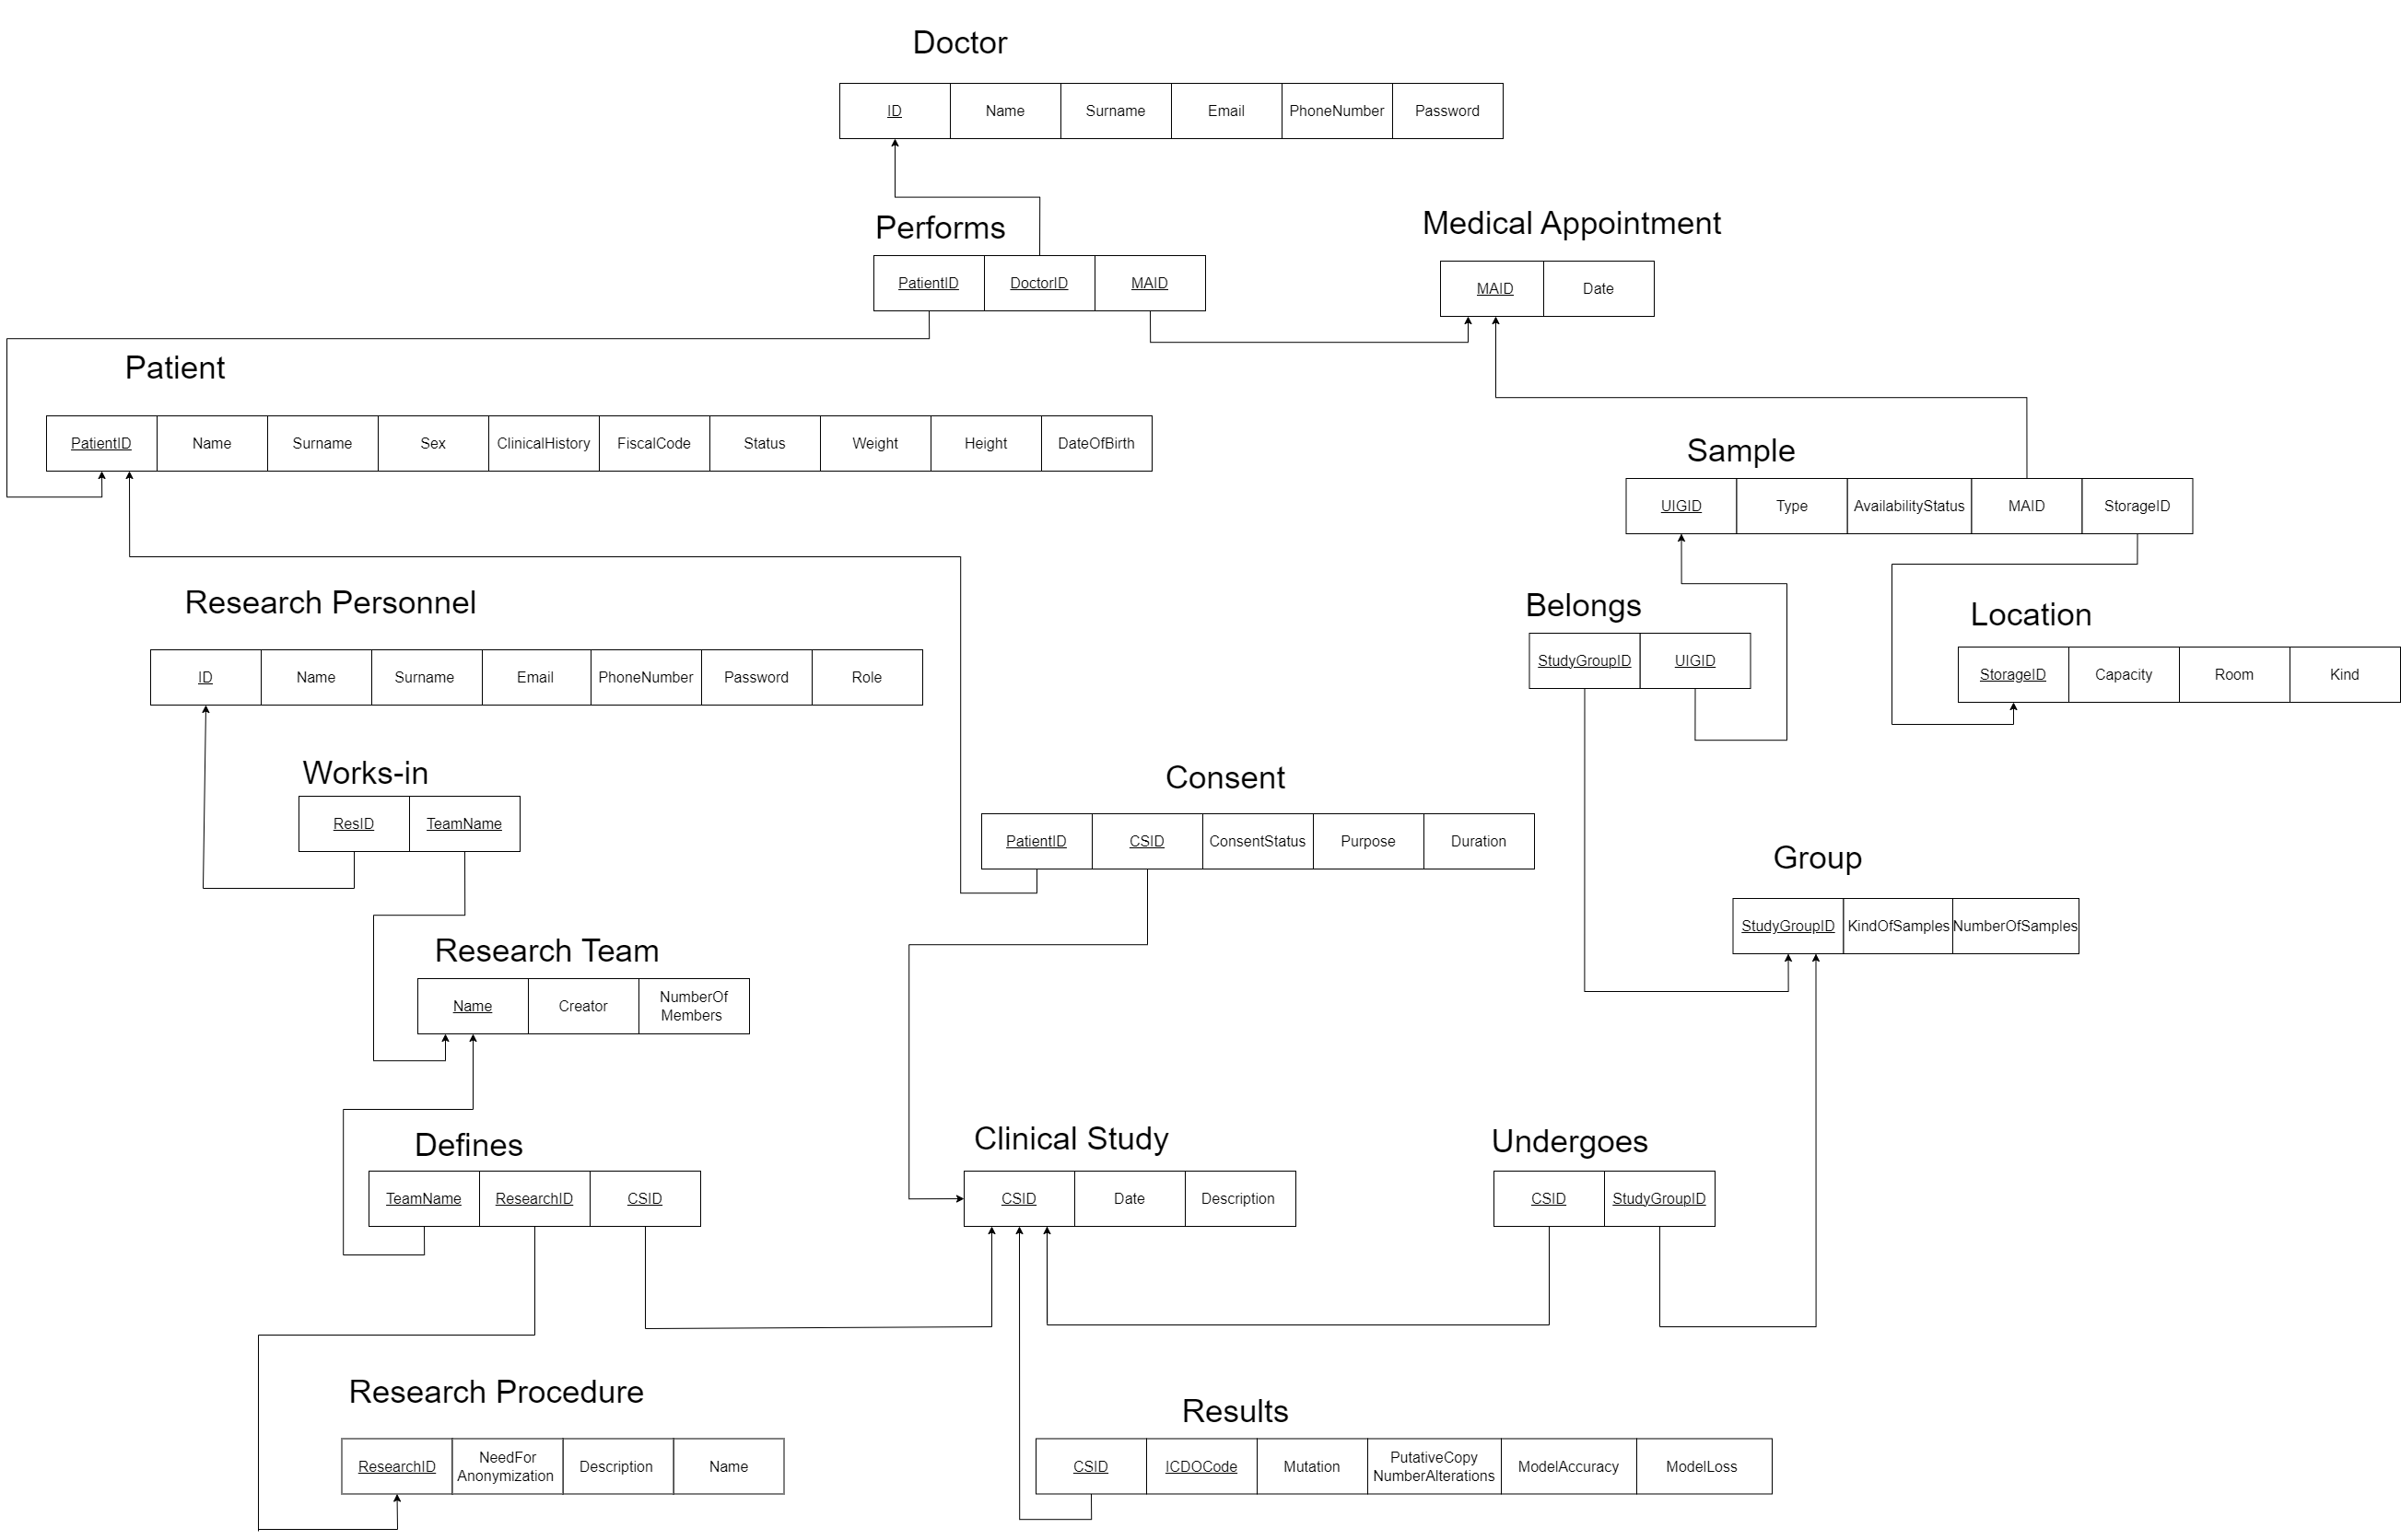
\includegraphics[width=\textwidth]{schemas/RelationalSchema.png}
    \caption{Relational Schema.}
\end{figure}
\end{center}

\newpage
